\documentclass[12pt, letterpaper, titlepage]{article}

\usepackage{amsmath, amsfonts}
\usepackage{booktabs}
\usepackage{amsthm}
\usepackage{graphicx}
\usepackage[margin=1in]{geometry}
\usepackage{hyperref}
\usepackage{cleveref}
\hypersetup{colorlinks = true, linkcolor = blue, citecolor=blue, urlcolor = blue}
\usepackage{natbib}
\usepackage{float}
\usepackage{setspace}
\usepackage{pdfpages}
\usepackage[pagewise]{lineno}
\usepackage{mwe}
\usepackage{comment}
%\linenumbers*[1]
% %% patches to make lineno work better with amsmath
\newcommand*\patchAmsMathEnvironmentForLineno[1]{%
 \expandafter\let\csname old#1\expandafter\endcsname\csname #1\endcsname
 \expandafter\let\csname oldend#1\expandafter\endcsname\csname end#1\endcsname
 \renewenvironment{#1}%
 {\linenomath\csname old#1\endcsname}%
 {\csname oldend#1\endcsname\endlinenomath}}%
\newcommand*\patchBothAmsMathEnvironmentsForLineno[1]{%
 \patchAmsMathEnvironmentForLineno{#1}%
 \patchAmsMathEnvironmentForLineno{#1*}}%

\AtBeginDocument{%
 \patchBothAmsMathEnvironmentsForLineno{equation}%
 \patchBothAmsMathEnvironmentsForLineno{align}%
 \patchBothAmsMathEnvironmentsForLineno{flalign}%
 \patchBothAmsMathEnvironmentsForLineno{alignat}%
 \patchBothAmsMathEnvironmentsForLineno{gather}%
 \patchBothAmsMathEnvironmentsForLineno{multline}%
}

% control floats
\renewcommand\floatpagefraction{.9}
\renewcommand\topfraction{.9}
\renewcommand\bottomfraction{.9}
\renewcommand\textfraction{.1}
\setcounter{totalnumber}{50}
\setcounter{topnumber}{50}
\setcounter{bottomnumber}{50}

\newcommand{\jy}[1]{\textcolor{blue}{JY: #1}}
\newcommand{\eds}[1]{\textcolor{red}{EDS: (#1)}}


\title{On Devon Allen's Disqualification at the 2022 Track and Field World
Championship} 

\author{Owen Fiore\\
%   \href{mailto:owen.fiore@uconn.edu}
% {\nolinkurl{owen.fiore@uconn.edu}}\\
  Elizabeth Schifano\\
  Jun Yan\\[1ex]
  Department of Statistics, University of Connecticut\\
}
\date{}

\begin{document}
\maketitle

%Abstract should be 200 words
%Devon Allen was disqualified in 2022... discussions about dq, talk methods and 
%models, venue effect, and conclusion
\begin{abstract}
  Devon Allen was disqualified in the Men's 110 meter hurdle final of the 2022
  Track and Field World Championships after registering a reaction time of 0.099 seconds, 0.001 
  seconds faster than what is allowed.  Following the games, bloggers on the running website 
  LetsRun scrutinized the results and performed non-statistical analysis of the data.
  They found that the reaction time data from the 2022 World Track Championships seemed to be faster 
  compared to the other datasets they looked at, but did not perform any meaningful statistical 
  analysis of the data.  This paper questions the reaction time disqualification barrier, which is
  currently 0.1 seconds to determine whether this is a reasonable threshold.
  We employ a generalized linear mixed model (GLMM) with a random effect term
  which will be referred to as the venue effect in order to try and model the
  data.  Additionally, we employ a signed-rank test for clustered data to compare
  reaction times for the same athletes at different competitions.
  This matter needs to be addressed because Devon Allen's disqualification could 
  be a problem that could continue to re-appear in future world championships.

\bigskip
\noindent{\sc Keywords}:
Reaction Time, Seiko, 

\end{abstract}

\doublespace

\jy{The bib file needs quality control. Practice my writing tips in the
  stat-wriging notes: chapter 2 on latex/bibtex.}

\jy{Go over the reference section to see what need to be changed in the bib source}

\jy{Turn on column numbers in your editor to keep line width under 80.}

\section{Introduction}
\label{sec:intro}


After coming in third in the 110 meter hurdles at the United States Track and 
Field Championships in Eugene Oregon at the end of June, Devin Allen was expected to
be a contender for the World Championships, which were scheduled for two months 
later, also in Eugene. At the World Championships, Allen made it through the 
heats and semifinals to reach the finals while posting reaction times of 0.123
in the heats and 0.101 in the semifinal.  Allen, who attended the University
of Oregon (Location of US World Championship and the World Championship) was
considered to be a favorite for the 110 meter hurdle after running 12.84 seconds
in early June; only 0.04 seconds away from the world record \citep{wa2022preview}.
Thus his disqualification by reacting in 0.099 seconds instead of 0.01 was met
with shock from both Allen and fans alike.  NBC, who was broadcasting the
championships in the United States, later uploaded a video to their YouTube
channel that show the disqualification and can be found here:
\url{https://www.youtube.com/watch?v=D6NXTMo-1yM}. The crowd erupted with jeers when
they found out that Allen was disqualified, angry at the result.  Had Allen 
reacted just 0.001 seconds slower he would have been allowed to compete and been 
spared waiting another two years until the next World Track and Field Championship.
An investigation into reaction times is also important because reaction times have
been shown to affect the overall time of the race \citep{delalija2008reaction}.
Thus, faster reaction times lead to faster overall times; which is the goal of
every sprinter who steps onto the track.


Allen's disqualification has been discussed extensively in online communities
such as \url{www.LetsRun.com}, a website that is part message board and part
news. The message board,
which functions similarly to Reddit is very active during important running
events, which include during the finals of major events such as
the Olympics and the World Track and Field Championships.  However, it is the
\jy{cite these blog articles formally}
news section of the website that generated articles such as ``Was Devon Allen
Screwed? There's At Least a 99\% That He Was" and ``The Data Keeps Pouring In and
It Continues to Look Bad For World Athletics and Great For Devon Allen".  Robert
Johnson, who created and runs the Letsrun website argued that there was an error
with the timing equipment at the 2022 Track and Field World Championship and
cited graphs, statistics such as median reaction time, and compared the reaction
times at the 2022 Track and Field World Championship \citep{johnson2022devon}. 


Reaction time in sprint and hurdle events has been studied by many authors.
\citet{pain2007sprint} looked at
reaction times for nine male athletes and analyzed their reaction times.  The
fastest athlete of the nine, had on average (even with their two fastest time 
removed) a reaction time of 0.087 seconds and a standard deviation of 0.004
seconds.  Two other athletes were able to react similarly when under certain
muscular tightening conditions.  In a study commissioned by IAAF,
\jy{define acronym at first occurrence}
\citep{komi2009iaaf} recommended that the disqualification 
barrier be decreased to allow sprinters to
react faster, and suggested 0.08 or 0.085 seconds as possible new thresholds.
Additionally, it was recommended to IAAF that high speed cameras be used to
change the reaction time criteria from pushing off on the block to body
movement. This could provide a more accurate representation of 
reaction time, and thus the possibility of a false disqualification would be lowered.
The possibility of using a video-based medium has been proved to be a reliable
measure of reaction time \citep{mudric2015evaluation}.


\jy{Could be condensed}
\citet{pilianidis2012start} found
significant differences between reaction times at several world championships
between 1997 and 2009 for the men's 110 meter hurdles.  Another important
conclusion was that for reaction times did not decrease over the twelve years
covered by the research in the study \citep{pilianidis2012start}.  This contradicts
what was found in a 2021 study that concluded the year of competition has a
significant effect on reaction times \citep{zhang2021correlation}.  Their
analysis looked at data from the 2011-2019 World Championships across multiple
sprint events and concluded that from 2011 to 2019, reaction times got
faster. However, not  all studies have been in favor of a decrease in the
reaction time barrier. \citet*{brosnan2017effects} in 2016 argue for increasing 
the reaction time barrier to 0.115 seconds, and cited evidence from European 
Championships and World Championships in their article.  A study looking 
at the 2008 Olympics likewise supported the conclusion that athletes could not
react in as little as 0.1 seconds \citep{lipps2011implications}.  Another study
concluded that visual reaction times to the starting gun may be faster by 0.007
seconds than the IAAF method, which is from force on block starts 
\citep{holmes2018method}.  While this may seem trivial, Allen was disqualified
only by 0.01 seconds. It is also worth noting that one study looking at data 
from various IAAF meets found that the fastest reaction times for men were found
between the ages of 26 and 29 \citep{tonnessen2013reaction}.  This is notable 
because Allen was 27 years old at the 2022 Track and Field World Championship 
and in his physical peak.


\jy{language needs to be formalized and condensed.}
The objective to this paper is to analyze the reaction times at the 2022
World Track and Field Championship to check for any abnormalities, and we approach
this two different ways.  Our first method is to try to model the data, which is
the reaction times of every non-disqualification since the 1999 World Championships. 
The model we use is a gamma linear mixed-effects model with a random effect
accounting for the venue (or year) effect. 
The second method is to compare data for athletes who have competed
at additional competitions to see how their reaction times compare from previous
competitions to this one. First we can look at the reaction times of athletes who
competed at the World Track and Field Championship in both 2019 and 2022 and
compare the times, and secondly we can look at how athletes performed compared
to how they did at their national/qualifiers meet. In order to reduce any chances
of athletes improving reaction time, we can also look at data from qualifying meets.
Almost every athlete had to qualify by proving they are elite at the national level, 
usually by coming in at least fourth. Thus, data was compiled on athletes who competed
at the 2022 World Track and Field Championships on what these athletes also ran 
at their country's national championship. If there was any argument that athletes
have improved their reaction time from 2019 to 2022, it should now be considered
nearly null, as the national competitions took place between June and July 2022 
and the World Championships were in August. The equipment used to measure reaction
time cannot be guaranteed to be the same from national to international
competition, but the time span between meets has been reduced considerably.


The rest of this paper is as follows: Section~\ref{sec:Data} describes how data was
collected and begins to detail the generalized linear mixed-effect (GLMM)
model which is further developed in the
Section~\ref{sec:Methods}.  The signed-rank test analysis for the same athletes is
also included in Section~\ref{sec:Methods}.  Section~\ref{sec:Results}
section provides the probabilities from the methods section and the paper ends 
by questioning the reaction time barrier.  Lastly, section~\ref{sec:Discussion}
discusses the impact and limitations of the paper.


\section{Data} \label{sec:Data}

There are two types of data that is explored throughout this paper: data from
1999-2022 for every world championship, and data from athletes who competed
at both the 2019 and 2022 World Championships and 2022 national competitions
and the 2022 World Championship.  The first data set is used for the GLMM portion
of the paper, while the second data set is used for the rank based comparisons.

\subsection{World Championship}


\begin{figure}[tbp]
  \centering
  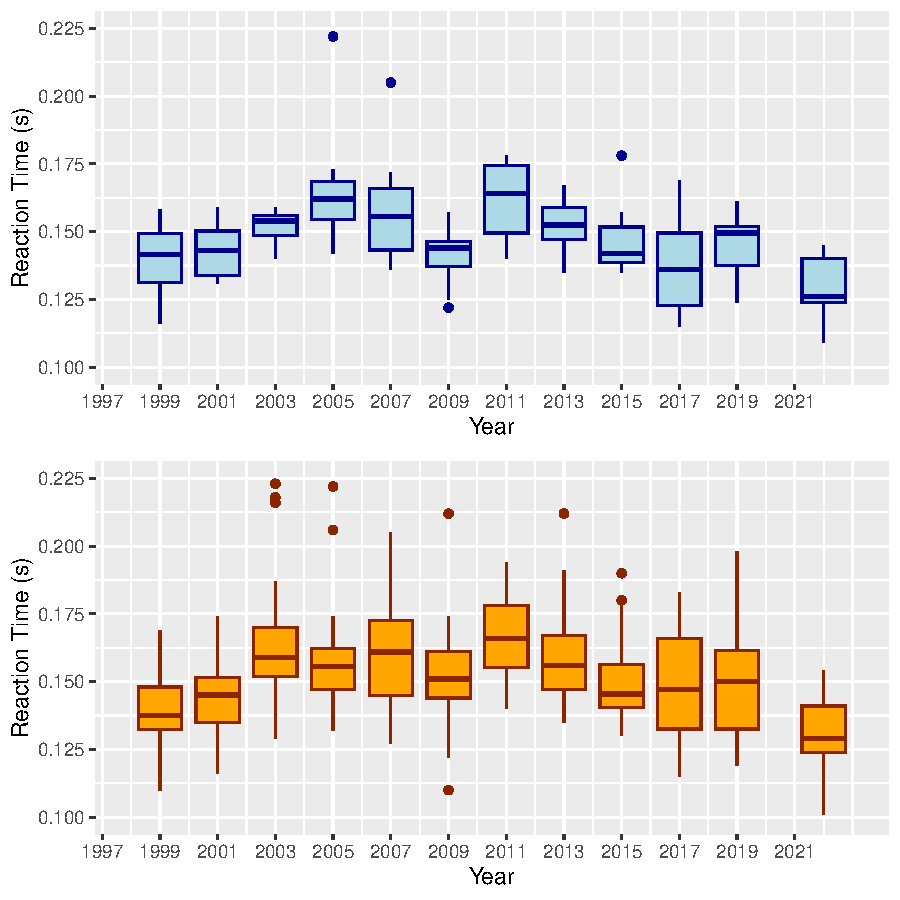
\includegraphics{Finals_Pooled_Boxplot}
  \caption{The reaction times from 2019 to 2022 for the men's final (top) and
  the men's semifinals and finals (bottom).}
  \label{fig:Boxplots}
\end{figure}

Data was taken from the World Athletics and covers the men's 110 meter hurdles 
and the women's 100 meter hurdles from 1999 to 2022.  The variable of prediction 
interest is reaction time, and the predicting variables are year, stage of 
competition (heats, semifinal, final), total time, and gender.  
The data can be found in the appendix~\ref{sec:Appendix}. Factors such as name, 
country, and identification number were not considered important for the 
purposes of this research besides the times for Devon Allen and the other 
United States athletes mentioned above.  The variable ``Stage"
refers to whether the observation occurred during the ``heats" (Preliminary round) which
is denoted by ``H" in the data, ``S" for ``semifinals" (Of which there are either 2 or 3 
heats each year), and ``F" for finals. The variable ``Gender" has levels ``M" and ``F" 
which stand for ``male" and ``female" respectively.  The variable ``Batch" takes a 
numerical value and every heat of every round from 1999 to 2022 was assigned it's
own number.  This was added because of suspected issues that reaction time may be
correlated with other runners reacting quickly (one runner reacting quickly may
result in other runners reacting quickly).  There is no statistical significance to
how the batches were labeled, they were ordered chronologically by meet but
reverse chronologically by year (Batch 1 is a preliminary Heat of 2022 and Batch
111 corresponds to the 1999 finals). Included are
box plots of the reaction times of the men's finals and the men's semifinals and
finals pooled together.  We will refer to the latter as the ``pooled data"
throughout the paper.  The heats or preliminary rounds were not studied because
athletes react faster as the competition progresses.  Athletes react faster in
the finals than the semifinals which are faster than the heats 
\citep{zhang2021correlation}.  If we want to determine if Allen's reaction time
is reasonable, then we thus need to look at the men's final data, with the men's
pooled data being included in order to increase the sample size.  In 2022, there
were only five data points due to two disqualifications and one athlete who 
qualified but did not compete.
The data that looked at in the paper is best visualized using a box plot as show 
in Figure~\ref{fig:Boxplots}.  It is clear that the 2022 box plot for both the
men's finals and semifinals data is lower (indicating a faster reaction time)
than in previous years.  The median for the men's pooled data in 2022 was 0.129
and the median for the men's final data in 2022 was 0.126.  For comparison,
Brosnan found reaction times of 0.156 seconds for men when looking at data from
1999 to 2014 \citep{brosnan2017effects}.


Something that is extremely important to note in the data is the inconsistency 
of World Athletics in terms of how they penalize false starts.  From 2007--2009,
the IAAF (the former name for World Athletics, and the governing body for the 
World Track and Field Champions) instituted a rule change that allowed one 
warning false start before a sprinter was disqualified \citep{iaaf2009falsestart}  This 
essentially gave sprinters a second chance and reduced the penalty for a false 
start.  There were 18 male and 7 female false starts at the 2007 World 
Championships, 18 male and 7 female starts at the 2009 World Championships. 
Starting in 2011, the rule was scrapped, and the old policy which automatically 
disqualifies runners who false start was reinstituted.  The effect? At the 2011 
World Championship there were 6 male disqualifications and 4 female 
disqualifications \citep{iaaf2009falsestart}. By returning to the harsher policy and 
cracking down on false starts, World Athletics had reduced the number of 
false starts by two thirds. One study that looked at different false start
rules that IAAF has imposed from 1997 to 2009 and found that the reaction 
times when there was less leniency improved by a statistically significant amount
\citep{haugen2013effect}. This was desirable for World Athletics as false starts can 
make already long track meets more tedious, both for athletes and viewers watching the 
television broadcast.  Since 2011, IAAF has instituted the one false start rule
\citep{iaaf2009falsestart}.  However, we chose not to include women's data in this
paper due to the numerous papers citing difference in reaction times in men and
women's reaction times: \citep{lipps2011implications, babicc2009reaction,
panoutsakopoulos2020gender}


\subsection{Beyond World Championship}
This section was motivated from a qualitative analysis that started by looking
at how United States athletes reacted at the 2022 United States Track and Field
Championships. From June 23-26 2022, USA held its Track
and Field Championship to decide who to send to the World Championships at Hayward 
Field, the exact same venue as used for the World Track and Field Championship a month 
later.  Thus, a baseline is able to be established for the four USA athletes who 
competed in at least one round of both events: Trey Cunningham, Daniel Roberts, 
Grant Holloway, and Devon Allen. Every athlete reacted faster in all the World 
Track and Field Championship races compared to the USA Track and Field 
Championship races. Devon Allen raced three times at the USA Track and
Field Championship and three times at the World Track and Field  Championship. 
His reaction times were significantly faster in the World Track and
Field Championship compared to the USA Track and Field Championship as were his
teammates.  This comparison suggests that the timing system used between the two
meets may have been meaningfully different to the point where Devon Allen was
disqualified more because of faulty equipment rather than because he reacted
\jy{cross-reference to the table by its label}
too quickly.  Table~\ref{fig:USAvsWorld} below highlights the difference in reaction times for
Devon Allen, Trey Cunningham, Grant Holloway, and Daniel Roberts. ``USA" denotes
the USA Track and Field Championships, ``World" denotes the World Track and Field
Championships,   All numbers listed in the table are the reaction
time for the respective athletes in seconds. 

\begin{table}
\begin{center}
  \begin{tabular}{c c c c c c c} 
   \toprule
   Athlete & USA H & USA S & USA F & World H & World S & World F \\ [0.5ex] 
   \midrule
   Devon Allen & 0.201 & 0.153 & 0.160 & 0.123 & 0.101 & 0.099 \\ 
   Trey Cunningham & 0.186 & 0.185 & 0.182 & 0.115 & 0.120 & 0.109 \\
   Grant Holloway & 0.192 & 0.190 & N/A & 0.147 & 0.128 & 0.124 \\
   Daniel Roberts & 0.181 & 0.200 & 0.183 & 0.179 & N/A & N/A \\ [0.5ex]
   \bottomrule
  \end{tabular}
  \label{fig:USAvsWorld}
  \caption{Rection times for four United States Athletes at the 2022 USA Track
  and Field World Championships and the 2022 World Track and Field Championship.
  ``N/A" was used for any athlete that did not compete and thus did not register 
  a reaction time.}
  \end{center}
\end{table}

This dataset is quite small to perform any formal statistical analysis on, but
the data was expanded to include data for athletes who competed at national
competitions (many of which were held from May-July of 2022).  Once the data
was collected, each athlete was designated to be a cluster and the stage of
competition (national or international) was specified to be the group. 

\section{Methods} \label{sec:Methods}

The World Championship data and the data beyond the World Champisonship were
analysed with GLMM and rank-based approaches, respectively.

\subsection{GLMM}
Based on an exploratory analysis, the GLMM model that we chose was a gamma
mixed-effect model for the reaction times from the World Championship. The
normal error model on the log-scale was found to be inferior to the gamma model.
Let $Y_{ij}$ be the reaction time of observation~$j$ in year~$i$.
Conditional on a venue effect $z_i$ of year~i,  $Y_{ij}$ is modeled by a
gamma distribution with mean
\[
\mu_{i} = \alpha + z_i,
\]
and variance
\[
\sigma_i
\]
...
\jy{need to add assumptions ...}






The R package \texttt{lme4} allows various linear mixed effects models to be created, and 
was the primary modeling package used for our data analysis \citep{lme4}.
A gamma mixed linear effects model was chosen as the best model to model the data.
Many models were tried and compared to determine what the strongest model.  For
a fixed data set such as the men's pooled data including 2022, the models with
the venue effect included performed better than the models without the venue
effect for each set of comparable models; as indicated by the lower AIC and
higher log likelihood.  Thus, the venue effect is significant and should be
included in the model.  It can also be established that a gamma distribution
better models the data than linear data from comparing the linear model with
venue effect and them gamma model with a venue effect.  The final decision that
was made in model selection was to include link = log in the model.  Despite
doing very little to alter the AIC or log likelihood, the log scale was included
in order to try and better deal with high outliers. %Include Residuals plot?

Once the Gamma mixed effects model was chosen, it needed to be decided which combination
of effects to use.  It was possible to include a venue effect, a batch effect, 
or a year and batch effect.  The batch effect is very
difficult to explain or interpret as it means that some heats of races were either
faster or slower and that everyone in the batch reacted similarly.  Although
it is possible that one athlete reacting faster could lead to others reacting
similarly, this does not make much practical sense as the difference between
heats that had fast and slow reaction times are all within 0.12 seconds of each
other.  It is much easier however to explain the venue effect.  The technology
that World Athletics has used has differed since 1999 and theoretically the
reaction time data from 2022 should be the best as the timing system should be
state of the art.  Any other weather or climate related factors such as humidity,
precipitation, elevation, etc. would all be negated when looking at the batch
effect, but are all factors that could potentially impact the venue effect.


%Throughout exploratory analysis, gamma provides better AIC
%Spend paragraph on after fitting the model how to figure out 0.1 p value
As the GLMM model has mixed form, the best way to try to gauge the probability
of observing a reaction time is to simulate the distribution of times using a 
large sample.  In order to approximate the distribution, R code was written to 
try and estimate the probabilities of observing a reaction time as extreme as
0.1 seconds.  The code re-paramertizes the gamma distribution to be in terms of
$\mu$ and shape rather than by $\alpha$ and $\beta$.  From the code, it is
possible to calculate the probability of observing a reaction time faster than
a given time.  We want the probability of a reaction time being less than 0.1
seconds in order to gauge if that is a reasonable disqualification barrier.


%T, generate from fitted model explain what
%The R code does.  Simulate from fitted model. Use distribution of model to 
%Figure out the p value of reaction time less than 0.1



\subsection{Rank-based Comparison}


%Citations needed
%Include math formulas and the test statistic
%Equation of test statistic is from papers cited by clusrank. Asymptootic dist
%Was found by __ referecne and the implementation is from the clusrank R package


\jy{Undefined notations}
The test statistic of the DS method of the Wilcoxon rank-sum statistic is:
$Z = \frac{S - E(S)}{\sqrt{\hat{\text{Var}}(S)}}$ where 
$W^* = \frac{1}{N} + \sum_{i=1}^{N} \delta_{i}^{*} R_{i}^{*}$, $R_{i}^{*}$ is
the rank of $X_{i}^{*}$. S is given as $S = \mathbb{E}[W^* | X, \delta]$ and
$E(S) = E(W^*) = \frac{1}{2} \sum_{i=1}^{N} \frac{n_i}{N}$.
The asymptomatic distribution of the Wilcoxon rank-sum statistic was found by
\citet{datta2005rank} and the R package ``clusrank" allows for its implementation.
\citep{jiang2017wilcoxon}.
---Please see manuscript around line 464 for comments regarding this section---

%I included additional statistics from the paper, I am unsure of how in depth
%This explanation needs to be


%$F_{i}(x) = \frac{1}{n_i} \sum_{k=1}^{n_i} \mathbb{I}(X_{i,k} \leq x)$

%$F_{i}(x-) = \frac{1}{n_i} \sum_{k=1}^{n_i} \mathbb{I}(X_{i,k} < x)$

%$S = \frac{1}{N + 1} \sum_{i=1}^{N}  \sum_{k=1}^{n_i} \frac{\delta_{ik}}{n_i} \left[ 1 + \frac{1}{2} \sum_{j \neq i} \frac{1}{n_j}
%\left( F_j(X_{ik}) + F_j(X_{ik-}) \right) \right]$






Using the \texttt{clusWilcox.test()} function, a Wilcoxon rank sum
test was performed with the cluster set to be the Athlete and group set to Year
using the DS method. The DS method is preferable when the cluster sizes are
informative \citep{jiang2017wilcoxon}.  In this case, athletes who have more
data are generally thought to be faster, as they have made it further in the
competition.  Clusters range from two to six, with two indicating that at each
competition they only made it to the heats, but a cluster size of six indicates
that they made the finals in both competitions.  While the number of times
athletes compete is based off their overall time not their reaction time, the
two are correlated \citep{delalija2008reaction}.


\section{Results} \label{sec:Results}

\subsection{GLMM} \label{subsec:Results_GLMM}
%Section 4.1: Gamma model results show the fitting with and without 2022,
%talk about p values and thresholds from the simulations (do not include the
%results in the methods section).

\jy{present the estimated parameters first before deriving the p-value using the
  estimated parameters. The difference in variance of the random effects using
  different data motivated the rank-based study.}

As shown in table~\ref{tab:Gamma_parameters}, the standard error of the year
effect increases for both the men's final and men's pooled data sets when
including 2022.  The men's final data venue effect error increased from 0.439
to 0.504 and from 0.0495 to 0.0554 for the men's pooled data.  This demonstrates
that the inclusion of 2022 increased the randomness of the data and motivates
the rank-based study~\ref{subsec:Results_Rank}.

\begin{table}
  \centering
  \begin{tabular}{c c c c c c}
      \toprule
      Dataset & Venue standard error & Int effect est & Int se & Int var & Resid Var \\
      \midrule
      Older Finals & 0.0439 & $-1.901$ & 0.0251 & 0.0019 & 0.0109 \\
      All Finals & 0.0504 & $-1.914$ & 0.0280 & 0.0025 & 0.0112 \\
      Older Pooled & 0.0495 & $-1.853$ & 0.0305 & 0.0024 & 0.0243 \\
      All Pooled & 0.0554 & $-1.869$ & 0.0348 & 0.0031 & 0.0235 \\
      \bottomrule
  \end{tabular}
  \caption{Summary statistics for the GLMM on various data sets}
  \label{tab:Gamma_parameters}
\end{table}

At a size of $n=10,000,000$, the calculated probability of a reaction
time being below 0.1 seconds was as follows for the various different data sets:
\jy{label the table and reference to it; clean it up}
\begin{table}
  \centering
  \begin{tabular}{c c c c} 
   \toprule
   Data Set & P(RxnTime $<$ 0.1) & P(RxnTime $<$ 0.09) & P(RxnTime $<$ 0.08) \\ 
   \midrule
   all finals gamma log & $8.56\cdot10^{-4}$ & $4.1\cdot10^{-5}$ & $6.0\cdot10^{-7}$ \\ 
   old finals gamma log & $4.39\cdot10^{-4}$ & $1.63\cdot10^{-5}$ & $2.0\cdot10^{-5}$ \\
   all pooled gamma log & $6.86\cdot10^{-3}$ & $1.21\cdot10^{-3}$ & $1.3\cdot10^{-4}$ \\
   old pooled gamma log & $5.76\cdot10^{-3}$ & $9.93\cdot10^{-4}$ & $1.0\cdot10^{-4}$\\
   \bottomrule
  \end{tabular}
  \caption{Probabilities of observing reaction times less than 0.1, 0.09, and
  0.08 for various data sets}
  \label{tab:Sim_probability}
\end{table}

Using the gamma function with link set to log, the probability of the function being
less than 0.1 seconds can be calculated to see if Allen's disqualification was an anomaly.
Prior to the 2022 World Championship, there was a 0.0439\% chance (based on the
simulated results) of observing a reaction time below 0.01 seconds in the men's
finals as shown in table~\ref{tab:Sim_probability}.
That means that we would expect a time below the threshold to occur
once every 2,277 starts.  Considering there are roughly 8 men's finals reaction
times every 2 years (The World Championship is biennial), every 569 years there
should be a time as extreme as Allen's.  This seems extremely unlikely, and thus
it seems like there may be an additional explanation for the fast reaction times.


It is interesting that the probability of observing a reaction time below 0.1
seconds increases drastically for the finals data and increases by a smaller margin
for the pooled data set after 2022 is included in the data set.  By including 2022
in the data, the chances of observing an extreme time are increased, showing that
2022 is a high outlier for reaction times compared to other years.


Table ~\ref{tab:Sim_probability} shows that changing the reaction time barrier from 0.1 seconds to
0.08 seconds drastically reduces the chances of observing a reaction time that
would break the barrier.  For the dataset of all finals data, the probability
associated with observing a reaction time below 0.08 seconds was $6\cdot10^{-7}$.
If IAAF were to change the reaction time the way that \citet{komi2009iaaf}'s paper
suggests, the probability would be so much lower that athletes would likely not
have a case to make when arguing against a disqualification.

%Discussion should show that random effect
%and standard error increase and that 2022 is special.  Now talk about Seiko
%timing equipment

%Citation needed in this section
Since 1985 Seiko Holding Corporations has served every World Athletics Championship
as the official timer \citep{wa2022seiko}.  Since 1985, the technology and the ability
to accurately predict measurements: long jump distances, false starts, total time,
reaction time, etc. have all dramatically improved.  Seiko did not start tracking
reaction time as an official measurement until 1999 in the men's and women's 100 meter
hurdles.  Seiko regularly updates their equipment so that they provide cutting edge
technology to the World Track and Field Championships, the highest stakes in the world
of running outside of the Olympics. Seiko's technology for detecting reaction 
times relies on the pressure that athletes
exert on the plate when they push off.  Their systems measure the time differential
between when the ``gun" goes off to start the race and when the pressure changes 
\citep{wa2022seiko}  If an athlete has a reaction time under 0.10 seconds, it is deemed a 
false start as it is considered that no athlete can react so quickly 
\citep{Seiko-Timing}.  Thus, a reaction time of for example 0.05, suggests that 
the athlete predicted the gun and it was luck that caused their abnormally high 
time.  At the World Championship level, World Athletics and Seiko want to remove 
that element of luck and thus impose the 0.1 second barrier. In 2013, Seiko 
upgraded their timing equipment for sprinting events (100 meter hurdles falls 
under this category) \citep{wa2013backtage}.  Since 1999, the highest reaction 
times in the men's 110-meter hurdle were recorded in 2013.  That is not to say that the higher 
times were caused by Seiko's equipment, but the two may be related.  It is worth noting that prior
to 2022, Seiko again upgraded its technology but for its jump management system.


\subsection{Rank-based Comparison} \label{subsec:Results_Rank}
%Section 4.2 is motivated by seiko timing and look at same athletes across
%multiple types of competition: 2019 and national

%Discussion/Conclusion is beyond results.  Limitations, what type of data we
%hope to have.

When the clusrank rank sum test was performed, the ``ds" method produced a z score of
2.9751 and p value of 0.001464.  This value is for a one-sided test and show that
the mean reaction time on average in 2019 was larger than the mean reaction time
in 2022 for athletes who competed in both championships at an alpha level of 0.01.
This provides good evidence that athletes who competed in both 2019 and 2022 got
faster during that timespan.


Repeating the data collection steps and
again performing a clustered analysis for a Wilcoxon ranked sum test
results in two new z scores and p values.  The ``ds" method produced a z score of
3.6069 and p value of 0.000155.  This result is highly significant and shows that
the times at the national stage of competition were significantly higher than
the reaction times at the World Championships even for an alpha level of 0.001.

As Seiko timed both events, there should not be a significant
difference if the timing equipment in both instances was working correctly.
  To put it simply, there is not a reasonable explanation for 
this. It is inconceivable that so many athletes would improve such a significant
amount in such a small amount of time. 6 countries are represented in this 
comparison, which drastically decreases the chances of this issue being caused by
one specific country.  The United States athlete's improvement in times was
discussed earlier in the paper, but this data shows that on average there was
%Use a reference in this part
improvement for British, Polish, French, Brazilian, and Spanish athletes.


\section{Discussion}\label{sec:Discussion}

One conclusion from \citet{zhang2021correlation}'s analysis was that athletes
reaction times improved from 2011 to 2019.  However this study does not consider 
data from 1999 to 2009, and over this timespan athletes get slower and then
faster.  A boxplot~\ref{fig:Boxplots} shows that for the men's pooled data, the 
year with the fastest median reaction time before 2022 was 1999.  Thus, this 
reject's Zhang's conclusion that athletes are getting faster because they were 
fast over twenty years ago. One possible explanation for why 2011 had such
high variation was because of the IAAF rule discussed earlier that increased the
penalty of a false start to an instant disqualification \citep{iaaf2009falsestart}.
Athletes may have been overly cautious to false start and may have consciously
or sub-consciously reacted slower as a result.  Instead, a more appropriate 
conclusion may be that there is a lot of variability in reaction times and that
the context behind the races matters.

It is worth noting that in the semi-finals of the World Track and
Field Championships; Allen's reaction time was 0.101 which is only 0.001 above
the legal limit.  What this suggests is that Allen may have strong reflexes
and be able to react extremely well to the sound of the gun.  It seems unlikely that
Allen would be able to correctly predict the gun with such precision two times in a row,
which is the exact reason that the 0.10 second reaction time disqualification barrier was
imposed in the first place.  But Allen showed that at the Championship he was able to
react extremely fast two times, which may suggest skill rather than luck. Devon 
Allen is a very good athlete, as evidenced by his football career at the University of Oregon
and making it onto the Philadelphia Eagles practice squad this past year 
\citep{hurley2022eagles}. Thus, the 0.099 reaction time may not have been 
a product of Devon Allen predicting the start of the race but rather a 
combination of a quick reaction and a possibly faulty sensor.

Devon Allen's disqualification at the World Track and Field Championships was
possibly the result of both a faulty timing equipment and Devon Allen
reacting extremely quickly to the start.  The code and data from R showed that
the 2022 World Track and Field Championships were a low outlier compared to
every other year in terms of average reaction time.  Additionally, it was shown
through a gamma mixed effects model that there are significant year and batch
effects that greatly impact reaction time.  However, this practically does not make much sense
as there is no reason for so much random variation without much of a trend.
There has not been a consistent decrease or increase since 1999, much of the data
for reaction times has been random and unpredictable.  Thus while it seems easy
to conclude that Devon Allen was wrongly disqualified, that may not necessarily
be the case.  If there are issues with reaction time such as athletes approaching the 0.10 
second barrier again at the next World Track Championship (August 2023), then World Athletics 
needs to adjust that threshold and allow for faster reaction times so that athletes with superb 
reflexes are not penalized like how Allen was in 2022.  World Athletics did not
do anything about \citet{komi2009iaaf}'s study, but perhaps they should now so
that the story of Devon Allen is not repeated.

This paper does not consider data from the women's 100 meter hurdle, and although
that was initially because of concerns over reaction time differences in men and
women, exploratory analysis was performed and showed that 2022 was at best only
slightly faster relative to other championships going back to 2022.  Likewise,
the rank based comparisons results in p values that were not significant.  The
lack of evidence from looking at the women's data makes it harder to conclude 
that the sensors used at the 2022 championships were faulty, although it is
unknown if the sensors for the men's 110 meter hurdle and women's 100 meter
hurdle were the same.

\section{Appendix}
\label{sec:Appendix}
%Put downloadable data spreadsheet
Here is World Athletics website with the data: \url{https://www.worldathletics.org/results/world-athletics-championships}.
Here is the data for the USA Track and Field Championships: \url{https://www.flashresults.com/2022_Meets/Outdoor/06-23_USATF/}

For the pooled data set
\begin{center}
  \begin{tabular}{|c  c  c  c  c  c  c |}
   \hline 
   Model & AIC & Log Likelihood & Int effect est & Int se & Int var & Resid Var \\ [0.5ex] 
   \hline\hline
   linear one & -1667 & 835.5 & 0.1529 & 0.0014 & N/A & N/A \\
   \hline
   linear year & -1713 & 859.3 & 0.1541 & 0.0040 & 1.719e-04 & 5.926e-04 \\ 
   \hline
   gamma one & -1756 & 880.2 & 6.554 & 0.0598 & N/A & N/A \\
   \hline
   gamma year & -1848 & 926.9 & 6.553 & 0.2269 & 0.1305 & 0.0234 \\
   \hline
   gamma one log & -1756 & 880.2 & -1.880 & 0.0091 & N/A & N/A \\
   \hline
   gamma year log & -1848 & 927.0 & -1.869 & 0.0348 & 0.0031 & 0.0235 \\ [0.5ex]
   \hline
  \end{tabular}
  \end{center}

\bibliographystyle{chicago}
\bibliography{citations.bib}


\end{document}

Here are important statistics grouped by both model and data set:
All Men final's Data
\begin{center}
  \begin{tabular}{|c | c | c | c | c | c | c |} 
   \hline\hline
   Model & AIC & Log Likelihood & Int effect est & Int se & Int var & Resid Var \\ [0.5ex] 
   \hline
   linear one & -472.7 & 238.3 & 0.1484 & 0.0019 & N/A & N/A \\ 
   \hline
   linear year & -468.7 & 237.4 & 0.1481 & 0.0030 & 7.762e-05 & 2.457e-04 \\
   \hline
   men finals one gamma & -477.3 & 240.7 & 6.738 & 0.0844 & N/A & N/A \\
   \hline
   men finals year gamma & -491.1 & 248.5 & 6.8121 & 0.1895 & 0.1148 & 0.0112 \\
   \hline
   men finals one gamma log & -477.3 & 240.7 & -1.908 & 0.0125 & N/A & N/A \\
   \hline
   men finals year gamma log & -491.0 & 248.5 & -1.914 & 0.0280 & 0.0025 & 0.0112 \\ [0.5ex]
   \hline
  \end{tabular}
\end{center}

Pre-2022 final's data
\begin{center}
  \begin{tabular}{|c | c | c | c | c | c | c |} 
   \hline\hline
   Model & AIC & Log Likelihood & Int effect est & Int se & Int var & Resid Var \\ [0.5ex] 
   \hline
   linear one & -450.7 & 227.4 & 0.1495 & 0.0019 & N/A & N/A \\
   \hline
   linear year & -444.1 & 225.0 & 0.1496 & 0.0028 & 5.691e-05 & 2.470e-04 \\ 
   \hline
   gamma one & -455.8 & 229.9 & 6.687 & 0.0834 & N/A & N/A \\
   \hline
   gamma year & -465.1 & 235.5 & 6.714 & 0.1674 & 0.0859 & 0.0109 \\
   \hline
   gamma one log & -455.8 & 229.9 & -1.900 & 0.0125 & N/A & N/A \\
   \hline
   gamma year log & -465.0 & 235.5 & -1.901 & 0.0251 & 0.0019 & 0.0109 \\ [0.5ex]
   \hline
  \end{tabular}
  \end{center}

All Men's semifinal and finals data
\begin{center}
  \begin{tabular}{||c | c c c | c c c||} 
   \hline
   Athlete & USA H & USA S & USA F & World H & World S & World F \\ [0.5ex] 
   \hline\hline
   Devon Allen & 0.201 & 0.153 & 0.160 & 0.123 & 0.101 & 0.099 \\ 
   \hline
   Trey Cunningham & 0.186 & 0.185 & 0.182 & 0.115 & 0.120 & 0.109 \\
   \hline
   Grant Holloway & 0.192 & 0.190 & N/A & 0.147 & 0.128 & 0.124 \\
   \hline
   Daniel Roberts & 0.181 & 0.200 & 0.183 & 0.179 & N/A & N/A \\ [0.5ex]
   \hline
  \end{tabular}
  \end{center}

Pre-2022 Men's semi finals and finals data
\begin{center}
  \begin{tabular}{|c | c | c | c | c | c | c |} 
   \hline
   Model & AIC & Log Likelihood & Int effect est & Int se & Int var & Resid Var \\ [0.5ex] 
   \hline\hline
   linear one & -1539 & 771.5 & 0.1544 & 0.0015 & N/A & N/A \\
   \hline
   linear year & -1564 & 785.4 & 0.1562 & 0.0037 & 1.280e-04 & 6.273e-04 \\ 
   \hline
   gamma one & -1626 & 814.9 & 6.475 & 0.0608 & N/A & N/A \\
   \hline
   gamma year & -1688 & 846.8 & 6.426 & 0.1923 & 0.0989 & 0.0243 \\
   \hline
   gamma one log & -1626 & 814.9 & -1.868 & 0.0094 & N/A & N/A \\
   \hline
   gamma year log & -1687 & 846.6 & -1.853 & 0.0305 & 0.0024 & 0.0243 \\ [0.5ex]
   \hline
  \end{tabular}
  \end{center}



Sorted By Model instead:
Linear Model with no venue effect
\begin{center}
  \begin{tabular}{|c | c | c | c | c | c | c |} 
   \hline
   Dataset & AIC & Log Likelihood & Int effect est & Int se \\ [0.5ex] 
   \hline\hline
   All Finals & -472.7 & 238.3 & 0.1484 & 0.0019 \\
   \hline
   Older Finals & -450.7 & 227.4 & 0.1495 & 0.0019 \\ 
   \hline
   All Pooled & -1667 & 835.5 & 0.1529 & 0.0014 \\
   \hline
   Older Pooled & -1539 & 771.5 & 0.1544 & 0.0015 \\
   \hline
  \end{tabular}
  \end{center}

Linear model with venue effect
\begin{center}
  \begin{tabular}{|c | c | c | c | c | c | c | c |} 
   \hline
   Dataset & AIC & Year se & Log Likelihood & Int effect est & Int se & Int var & Resid Var \\ [0.5ex] 
   \hline\hline
   All Finals & -468.7 & 0.0088 & 237.4 & 0.1481 & 0.0030 & 7.762e-05 & 2.457e-04 \\
   \hline
   Older Finals & -444.1 & 0.0075 & 225.0 & 0.1496 & 0.0028 & 5.691e-05 & 2.470e-04 \\ 
   \hline
   All Pooled & -1713 & 0.131 & 859.3 & 0.1541 & 0.0040 & 1.719e-04 & 5.926e-04 \\
   \hline
   Older Pooled & -1564 & 0.113 & 785.4 & 0.1562 & 0.0037 & 1.280e-04 & 6.273e-04 \\
   \hline
  \end{tabular}
  \end{center}

Gamma model with venue effect
\begin{center}
  \begin{tabular}{|c | c | c | c | c | c | c | c |} 
   \hline
   Dataset & AIC & Year se & Log Likelihood & Int effect est & Int se & Int var & Resid Var \\ [0.5ex] 
   \hline\hline
   All Finals & -491.1 & 0.3388 & 248.5 & 6.8121 & 0.1895 & 0.1148 & 0.0112 \\
   \hline
   Older Finals & -465.1 & 0.2930 & 235.5 & 6.714 & 0.1674 & 0.0859 & 0.0109 \\ 
   \hline
   All Pooled & -1848 & 0.3612 & 926.9 & 6.553 & 0.2269 & 0.1305 & 0.0234 \\
   \hline
   Older Pooled & -1688 & 0.3145 & 846.8 & 6.426 & 0.1923 & 0.0989 & 0.0243 \\
   \hline
  \end{tabular}
  \end{center}

Gamma model with venue effect and link=log
\begin{center}
  \begin{tabular}{|c | c | c | c | c | c | c | c |} 
   \hline
   Dataset & AIC & Year se & Log Likelihood & Int effect est & Int se & Int var & Resid Var \\ [0.5ex] 
   \hline\hline
   All Finals & -491.0 & 0.0504 & 248.5 & -1.914 & 0.0280 & 0.0025 & 0.0112 \\
   \hline
   Older Finals & -465.0 & 0.0439 & 235.5 & -1.901 & 0.0251 & 0.0019 & 0.0109 \\ 
   \hline
   All Pooled & -1848 & 0.0554 & 927.0 & -1.869 & 0.0348 & 0.0031 & 0.0235 \\
   \hline
   Older Pooled & -1687 & 0.0495 & 846.6 & -1.853 & 0.0305 & 0.0024 & 0.0243 \\
   \hline
  \end{tabular}
  \end{center}
